% Created 2026-08-05 mer 18:42
% Intended LaTeX compiler: pdflatex
\documentclass[11pt]{article}
\usepackage[utf8]{inputenc}
\usepackage[T1]{fontenc}
\usepackage{graphicx}
\usepackage{longtable}
\usepackage{wrapfig}
\usepackage{rotating}
\usepackage[normalem]{ulem}
\usepackage{amsmath}
\usepackage{amssymb}
\usepackage{capt-of}
\usepackage{hyperref}
\usepackage[newfloat]{minted}
\author{marco robba}
\date{\today}
\title{}
\hypersetup{
 pdfauthor={marco robba},
 pdftitle={},
 pdfkeywords={},
 pdfsubject={},
 pdfcreator={Emacs 30.2 (Org mode 9.7.29)}, 
 pdflang={English}}
\begin{document}

\tableofcontents

sas\#+title:Monitoraggio e gestione del traffico ferroviario Documentazione
// per mermid mettere il codice solo nel file .org e poi usare la foto del mermid compilato nel latex
C-c C-x v per aprire un'immagine linkata in emacs
C-c C-, per inserire un blocco di codice velocemente
C-c C-c per compilare il codice
\section{Introduzione Descrizione Generale}
\label{sec:orga12f82d}
Cio che è realizzato è al fine della gestione di una rete ferroviaria e, in particolare, la gestione
delle stazioni, dei treni che compongono tale rete.
La gestione della rete è fornita attraverso in un app web che fornisce il neccessarrio per il monitoraggio e l'amiinistrazione della rete
\section{Specifica}
\label{sec:orga1d172f}
Di Quanto il sistema è capace:
\subsection{Modellazione Per Casi D'uso}
\label{sec:orgd27f361}
\subsubsection{Diagramma dei casi d'uso}
\label{sec:org547fd1e}
\begin{enumerate}
\item Descrizione aggiuntiva
\label{sec:org23decc5}
\begin{center}
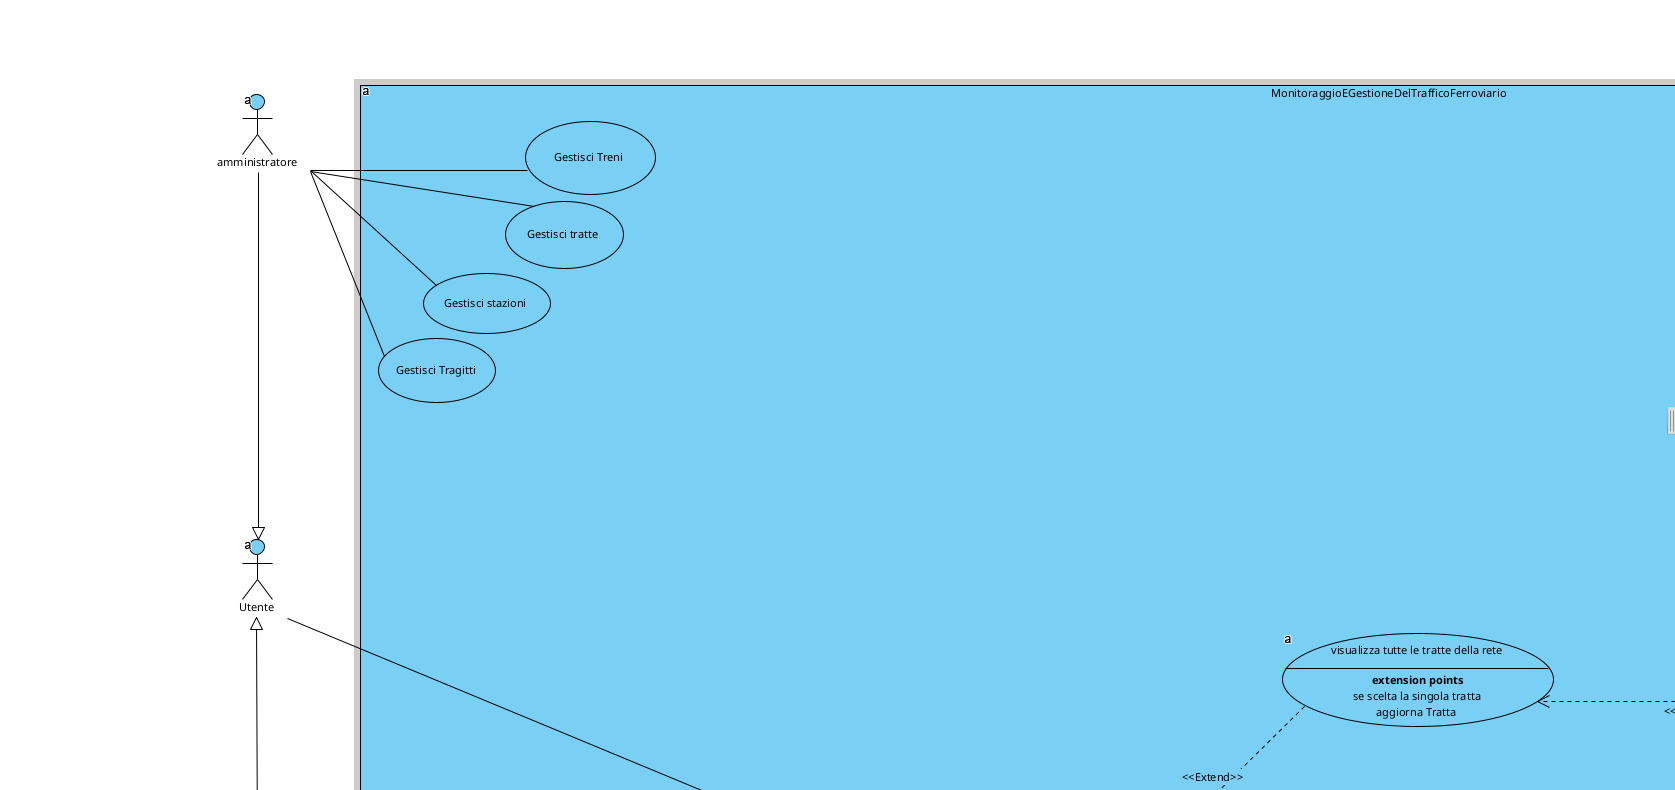
\includegraphics[width=.9\linewidth]{./immagini/diocane.png}
\end{center}
\begin{itemize}
\item gestisci <entità> indicherebbe crea enità, elimina entità, aggiungi entità, modifica entità
\end{itemize}
\end{enumerate}
\subsection{Elenco informale dei requisiti  funzionali}
\label{sec:org1b620d5}
\subsubsection{funzionalita da espletare per ogni componente}
\label{sec:org34c4676}
\begin{enumerate}
\item microservizio treno
\label{sec:orgcfabe83}
\begin{itemize}
\item aggiornamento tratta
\begin{itemize}
\item salvarla in ram per il proprio uso e sul db
\end{itemize}
\item gestione causa guasti alla prossima fermata stazione o binario (tratatta ovvero copia di stazioeni)
\begin{itemize}
\item ricezione dai sesori --> modifica della percorrenza della tratta, sincronizzazione sui topic di allarme delle
nuove stazioni
\begin{itemize}
\item se arrivano evendi del tipo la prossima stazione è fuori uso aggiornare variabile in rame e il database
che il treno si è femato e
\item se l'evento è il ripristino della funzionalità della stazione allora riaggiornare la ram e il db che il
treno è partito
\end{itemize}
\end{itemize}
\item Ritardi la tratta possiede orari corretti di percorrenza
\item inviare in certrale l'entrata e uscita da una stazione topic treni/+/passaggio
formato : boh lo fa l'ai
\item invio se il treno si guasta alla centrale
\end{itemize}
\item microservizio stazione
\label{sec:orgbc128d0}
\begin{itemize}
\item invio alla centrale i dati del passaggio dei treni
\begin{itemize}
\item i sensori della stazione informano id treno e se è in entrata o in uscita,
poi si aggiorna la ram e si inviano i dati alla stazione centrale per la storicizzazione
\end{itemize}
\item la staione può perdere la connessione
 con la centrale nel caso seguire il diagramma degli stati che ne
descrive la dinamica di gestione
\end{itemize}
\item Centrale
\label{sec:orgb2b18a9}
\begin{itemize}
\item deve rispondere alle richieste di visualizzazione
\begin{itemize}
\item montare su il motore in tepo reale, cicli continui che inviano i dati se la richiesta è ancora attiva
\end{itemize}
\item formattare e storicizzare i dati
\end{itemize}
L'unica crud a cui serve la propagazinone ai microservizzi è la
\begin{itemize}
\item gestione guasti
\begin{itemize}
\item se i microservizzi avvertono guasti , aggiornamento del db,
\item se il tecnico invia l'operatore aggiornare il db di modo che ormai il guasto sia terminato e
pubblicare sul topic degli allert generale per tutti i treni o tutte le stazioni che quel tale microservizio è stato risolto
\end{itemize}
\end{itemize}
interrogare il database ogni 10 secondi per ogni tipo di visualizzazione di modo da rendere il ``tempo reale''
\end{enumerate}
\subsection{Elenco maggiomente formale dei requisiti}
\label{sec:orgc11bb7f}
\subsection{Diagrammi degli stati}
\label{sec:org757ac07}
\subsubsection{Del Treno}
\label{sec:org2ddc77a}
\begin{enumerate}
\item Controllo e verifica Dell'id
\label{sec:org63645a7}
\begin{center}
\includegraphics[width=.9\linewidth]{/tmp/babel-KFq2Fi/plantuml-YhyHBy.png}
\label{}
\end{center}
\item Motore di simulazione del treno e stato di esso
\label{sec:org09f9c21}
\begin{itemize}
\item nota : gli stati del treno sono simulati, al posto delle simulazioni degli eventi nella realta tali dovrebbero essere implementati attraverso l'ascolto dei sensori di bordo
\end{itemize}
\begin{center}
\includegraphics[width=.9\linewidth]{/tmp/babel-KFq2Fi/plantuml-ayO21h.png}
\label{}
\end{center}
\end{enumerate}
\subsubsection{Della Stazione}
\label{sec:org5ec8781}
\begin{center}
\includegraphics[width=.9\linewidth]{/tmp/babel-KFq2Fi/plantuml-EDFLnw.png}
\label{}
\end{center}
\subsubsection{Del Server Centrale}
\label{sec:org32f08b4}
\begin{itemize}
\item nota: ci sono anche due macchine relative a stazione e treno sarebbero la proiezione lato della centrale operativa
\end{itemize}
\begin{enumerate}
\item mappa delle macchine
\label{sec:org82d0078}
\begin{center}
\includegraphics[width=.9\linewidth]{/tmp/babel-KFq2Fi/plantuml-RZwl9l.png}
\label{}
\end{center}
\item M1 ciclo di vita del processo della centrale
\label{sec:org4c4185d}
\begin{itemize}
\item e' la macchina radice: da qui partono in parallelo tutte le altre (main + TrafficLogicEngine.onStart)
\end{itemize}
\begin{center}
\includegraphics[width=.9\linewidth]{/tmp/babel-KFq2Fi/plantuml-BpFedx.png}
\label{}
\end{center}
\item M2 validazione dell'id dei nodi di campo
\label{sec:orgbd19f31}
\begin{itemize}
\item lato centrale della verifica dell'id gia' vista nei diagrammi del treno e della stazione (ExistIdForEdge / ExistIdForEdgeStazione)
\end{itemize}
\begin{center}
\includegraphics[width=.9\linewidth]{/tmp/babel-KFq2Fi/plantuml-dUuuq8.png}
\label{}
\end{center}
\item M3 ingestione della telemetria dei treni
\label{sec:org22b5774}
\begin{itemize}
\item consumo del topic railway/train/+/telemetry, aggiornamento della cache e storicizzazione solo al cambio di stato (IngestionService.onTelemetry)
\end{itemize}
\begin{center}
\includegraphics[width=.9\linewidth]{/tmp/babel-KFq2Fi/plantuml-89jLLp.png}
\label{}
\end{center}
\item M4 ingestione degli heartbeat delle stazioni
\label{sec:org00449d2}
\begin{itemize}
\item consumo del topic railway/station/+/heartbeat e chiusura automatica dei guasti aperti dal watchdog quando il battito torna (IngestionService.onHeartbeat)
\end{itemize}
\begin{center}
\includegraphics[width=.9\linewidth]{/tmp/babel-KFq2Fi/plantuml-T8dhjX.png}
\label{}
\end{center}
\item M5 ingestione dei transiti e dei passaggi
\label{sec:org7394366}
\begin{itemize}
\item lo stesso passaggio fisico arriva alla centrale da due strade, dal sensore di terra e dal treno: qui si vede chi fa cosa (onTransit / onPassaggio)
\end{itemize}
\begin{center}
\includegraphics[width=.9\linewidth]{/tmp/babel-KFq2Fi/plantuml-PsP2Eo.png}
\label{}
\end{center}
\item M6 ingestione degli allarmi dal campo
\label{sec:org25b3ba7}
\begin{itemize}
\item railway/alerts e' un topic condiviso, quindi la centrale deve filtrare i messaggi che ha pubblicato lei stessa (IngestionService.onAlert)
\end{itemize}
\begin{center}
\includegraphics[width=.9\linewidth]{/tmp/babel-KFq2Fi/plantuml-cXE0Xs.png}
\label{}
\end{center}
\item M7 ciclo di vita del guasto
\label{sec:org2f1ac00}
\begin{itemize}
\item macchina di entita': la storia di un singolo guasto, su cui agiscono M4, M6, M8 e M10
\end{itemize}
\begin{center}
\includegraphics[width=.9\linewidth]{/tmp/babel-KFq2Fi/plantuml-QN1fj0.png}
\label{}
\end{center}
\item M8 watchdog faultmonitor
\label{sec:org1a13803}
\begin{itemize}
\item i tre job schedulati ogni 10 secondi che rilevano cio' che i nodi di campo non possono segnalare da soli, cioe' la propria caduta (FaultMonitor)
\end{itemize}
\begin{center}
\includegraphics[width=.9\linewidth]{/tmp/babel-KFq2Fi/plantuml-PJwOpA.png}
\label{}
\end{center}
\item M9 sessione e autorizzazione delle api rest
\label{sec:org7e4a800}
\begin{itemize}
\item autenticazione tradizionale (variante 2 al posto di OAUTH2) e filtro dei permessi tecnico/amministratore su ogni chiamata
\end{itemize}
\begin{center}
\includegraphics[width=.9\linewidth]{/tmp/babel-KFq2Fi/plantuml-sqJ7DO.png}
\label{}
\end{center}
\item M10 gateway rest, crud e comandi operativi
\label{sec:orga8abd9a}
\begin{itemize}
\item ciclo di vita di una richiesta gia' autorizzata: letture, crud, comandi e notifiche verso il campo (RestApiGateway)
\end{itemize}
\begin{center}
\includegraphics[width=.9\linewidth]{/tmp/babel-KFq2Fi/plantuml-wTGoL0.png}
\label{}
\end{center}
\item M11 canale websocket realtime
\label{sec:orgac32fd3}
\begin{itemize}
\item punto di uscita comune di quasi tutte le altre macchine verso la dashboard (RealtimeWebSocket)
\end{itemize}
\begin{center}
\includegraphics[width=.9\linewidth]{/tmp/babel-KFq2Fi/plantuml-OMQaNJ.png}
\label{}
\end{center}
\item M12 stato runtime della stazione
\label{sec:org0e45d23}
\begin{itemize}
\item gli stati ONLINE / OFFLINE / GUASTA / MANUTENZIONE come li vede la centrale: stanno solo in cache, sul db ne resta la traccia nello storico
\end{itemize}
\begin{center}
\includegraphics[width=.9\linewidth]{/tmp/babel-KFq2Fi/plantuml-NwLUBK.png}
\label{}
\end{center}
\item M13 stato del treno
\label{sec:orgf59f9cf}
\begin{itemize}
\item proiezione sul database centrale della macchina a stati del convoglio: i quattro valori ammessi dal CHECK sulla colonna Treni.stato
\end{itemize}
\begin{center}
\includegraphics[width=.9\linewidth]{/tmp/babel-KFq2Fi/plantuml-qyol2x.png}
\label{}
\end{center}
\end{enumerate}
\section{Progettazione}
\label{sec:org6301482}
\subsection{Modello dati}
\label{sec:orgf36b0ca}
\subsection{Diagramma delle componenti}
\label{sec:orga98e713}
\begin{center}
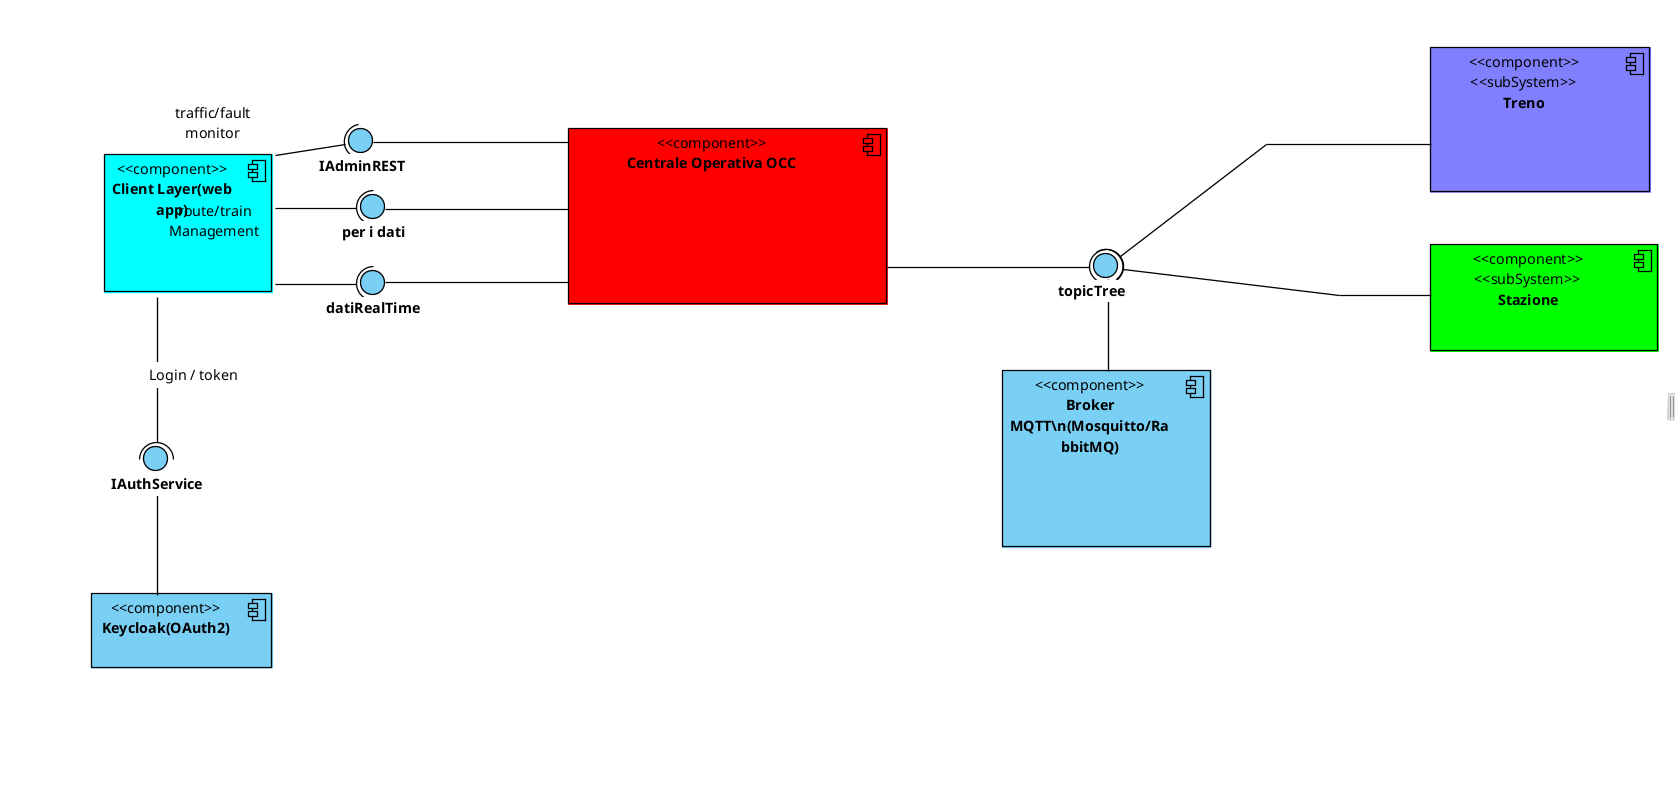
\includegraphics[width=.9\linewidth]{./immagini/diagrammaDelleComponenti.png}
\end{center}
\subsection{Diagramma di sequenza}
\label{sec:org1a5047a}
\end{document}
